%%%%%%%%%%%%%%%%%%%%%%%%%%%%%%%%%%%%%%%%%
% Journal Article
% LaTeX Template
% Version 1.4 (15/5/16)
%
% This template has been downloaded from:
% http://www.LaTeXTemplates.com
%
% Original author:
% Frits Wenneker (http://www.howtotex.com) with extensive modifications by
% Vel (vel@LaTeXTemplates.com)
%
% License:
% CC BY-NC-SA 3.0 (http://creativecommons.org/licenses/by-nc-sa/3.0/)
%
%%%%%%%%%%%%%%%%%%%%%%%%%%%%%%%%%%%%%%%%%

%----------------------------------------------------------------------------------------
%	PACKAGES AND OTHER DOCUMENT CONFIGURATIONS
%----------------------------------------------------------------------------------------

\documentclass[twoside,twocolumn]{article}

\usepackage{blindtext} % Package to generate dummy text throughout this template 

\usepackage[sc]{mathpazo} % Use the Palatino font
\usepackage[T1]{fontenc} % Use 8-bit encoding that has 256 glyphs
\linespread{1.05} % Line spacing - Palatino needs more space between lines
\usepackage{microtype} % Slightly tweak font spacing for aesthetics

\usepackage[english]{babel} % Language hyphenation and typographical rules

\usepackage[hmarginratio=1:1,top=32mm,columnsep=20pt]{geometry} % Document margins
\usepackage[hang, small,labelfont=bf,up,textfont=it,up]{caption} % Custom captions under/above floats in tables or figures
\usepackage{booktabs} % Horizontal rules in tables

\usepackage{lettrine} % The lettrine is the first enlarged letter at the beginning of the text

\usepackage{enumitem} % Customized lists
\setlist[itemize]{noitemsep} % Make itemize lists more compact

\usepackage{abstract} % Allows abstract customization
\renewcommand{\abstractnamefont}{\normalfont\bfseries} % Set the "Abstract" text to bold
\renewcommand{\abstracttextfont}{\normalfont\small\itshape} % Set the abstract itself to small italic text

\usepackage{titlesec} % Allows customization of titles
\renewcommand\thesection{\Roman{section}} % Roman numerals for the sections
\renewcommand\thesubsection{\roman{subsection}} % roman numerals for subsections
\titleformat{\section}[block]{\large\scshape\centering}{\thesection.}{1em}{} % Change the look of the section titles
\titleformat{\subsection}[block]{\large}{\thesubsection.}{1em}{} % Change the look of the section titles

\usepackage{fancyhdr} % Headers and footers
\pagestyle{fancy} % All pages have headers and footers
\fancyhead{} % Blank out the default header
\fancyfoot{} % Blank out the default footer
\fancyhead[C]{CCSU $\bullet$ GPG Protecting The First Amendment $\bullet$ CS 492} % Custom header text
\fancyfoot[RO,LE]{\thepage} % Custom footer text

\usepackage{titling} % Customizing the title section

\usepackage{hyperref} % For hyperlinks in the PDF

%----------------------------------------------------------------------------------------
%	TITLE SECTION
%----------------------------------------------------------------------------------------

%% \setlength{\droptitle}{-4\baselineskip} % Move the title up

%% \pretitle{\begin{center}\Huge\bfseries} % Article title formatting
%% \posttitle{\end{center}} % Article title closing formatting
%% \title{GPG Protecting the First Amendment} % Article title
%% \author{%
%%   \textsc{The application of encryption technology to protect citizens' constitutional rights}
%%   \thanks{Special Thanks to Jaine Tiu for her contributions and input in preparing this survey paper} \\[1ex] % Your name
%%   \normalsize Department Computer Science \\ Central Connecticut State University \\  Professor Vijayakanthan \\
%%   Undergraduate Student, K\\
%%   %%   \normalsize \href{mailto:khosro06001@gmail.com}{hos@ro.com} % Your email address
%% }


\setlength{\droptitle}{-4\baselineskip} % Move the title up
\pretitle{\begin{center}\Huge\bfseries} % Article title formatting
\posttitle{\end{center}} % Article title closing formatting
\title{GPG Protecting The First Amendment} % Article title
\preauthor{\begin{center}\lineskip 0.5em}
\postauthor{\end{center}}
\author{%
  \textsc{The application of encryption technology to protect citizens' constitutional rights}
  \thanks{Special thanks to CS undergraduate student Jaine Tiu for her invaluable contributions to the preparation of this paper.} \\[1ex] % Your name
  \normalsize Department Computer Science \\ Central Connecticut State University \\  Professor Vijayakanthan \\
  Undergraduate Student, K\\
  %%   \normalsize \href{mailto:khosro06001@gmail.com}{hos@ro.com} % Your email address
}



\date{\today} % Leave empty to omit a date
\renewcommand{\maketitlehookd}{%
  \begin{abstract}
    \noindent Tasked with exploring ethical and legal aspects of a timely and relevant
    subtopic of information security, and in this case
    GNU Privacy Guard (GPG)\cite{wikiGPG}, 
    we surveyed existing literature and assembled a cogent and logical database of facts
    that connect this technology to legal, ethical, and psychosocial aspects of its application.
    The focus of this paper in particular is the freedom to articulate opinions in digital format.
    We
    explored the relevance and utility of the application of GPG and cryptographic technology to the preservation of constitutional rights
    and finally suggested ways to pragmatically employ this technology for the benefit of society.
  \end{abstract}
}

%----------------------------------------------------------------------------------------



%\usepackage[english]{babel}			% english
\usepackage{graphicx}				% images
\usepackage{amssymb,amsmath}		        % math
%\usepackage{multicol}				% three-column layout
%\usepackage{url}					% clickable links
%\usepackage{marvosym}				% symbols
\usepackage{wrapfig}				% wrapping text around figures
%\usepackage[T1]{fontenc}			% font encoding
%\usepackage{charter} 				% Charter font for main content
%\usepackage{datetime}				% custom date
\usepackage{float}
\usepackage{placeins}
\usepackage{csquotes}

%% \usepackage{epigraph} %%% for quotes at the beginning of a chapter



%----------------------------------------------------------------------------------------

\begin{document}

% Print the title
\maketitle

%----------------------------------------------------------------------------------------
%	ARTICLE CONTENTS
%----------------------------------------------------------------------------------------

\section*{Introduction}

%%%\lettrine[nindent=0em,lines=3]{L} orem ipsum dolor sit amet, consectetur adipiscing elit.


\lettrine[nindent=0em,lines=3]{T}he very First Amendment to the US constitution protects Free Speech, to be more exact, it prohibits the US government from abridging the freedom of speech or the freedom of the press\cite{firstamendment}.
Indeed, it is the duty of the US government to protect
the right of individuals and
groups of individuals
to express their ideas, thoughts, and opinions
and to protect their right to freedom of assembly
- much less to censor or retaliate against them for exerting these rights.
The freedom to articulate and communicate one's thoughts and opinions,
regardless of the medium used for this purpose,
is even
expressly included as a
\textit{basic human right} in the
Universal Declaration of Human Rights \cite{humanrights}
and in the international human rights law.
Furthermore,
apart from protections guaranteed by the US constitution,
US case law provides ample evidence and support for this protection.
Once such precedence enshrined in the US case law, as
in Whitney versus California\cite{whitney},
Justia U.S. Supreme Court Center, 274 U.S. 357, in 1927:

\textit{
\enquote{
... to expose through discussion falsehood and fallacies, to avert the evil by the processes of education, the remedy to be applied is more speech, not enforced silence. -- Justice Brandeis }}

In other words,
the remedy for harmful speech is more speech, not enforced silence.

Voltaire once said:
\textit{``I disapprove of what you say, but I will defend to death your right to say it,''}
George Orwell describes freedom in the following fashion:
\textit{ ``If liberty means anything at all, it means the right to tell people what they do not want to hear,''}
and
Martin Luther King Jr. formulated the importance of the right to protest tyrannical governments as
\textit{``Somewhere I read of the freedom of speech. Somewhere I read of the freedom of the press. Somewhere I read that the greatness of America is the right to protest for right.''}
And, when it comes to tyrannical governments using the excuse of ``national security'' to squash dissent, freedom of speech, and other freedoms,
Ben Franklin poignantly asserted:
\textit{``Those who would give up essential Liberty, to purchase a little temporary Safety, deserve neither Liberty nor Safety.''}

During the Nuremberg trials, Herman Goering revealed:
\textit{``Of course the people don't want war. But after all, it's the leaders of the country who determine the policy, and it's always a simple matter to drag the people along whether it's a democracy, a fascist dictatorship, or a parliament, or a communist dictatorship. Voice or no voice, the people can always be brought to the bidding of the leaders. That is easy. All you have to do is tell them they are being attacked, and denounce the pacifists for lack of patriotism, and exposing the country to greater danger.''}\cite{goering}



\begin{figure}
\centering
  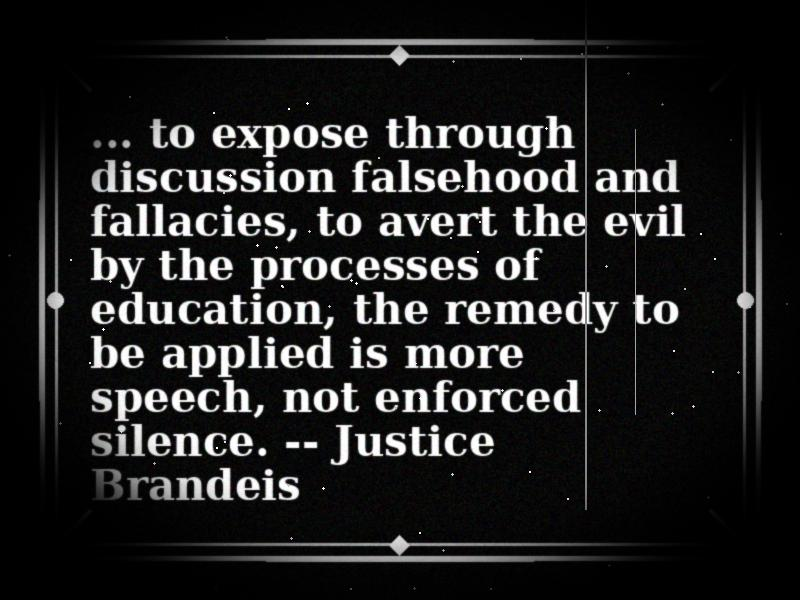
\includegraphics[width=0.45\textwidth]{i/brandeis.jpg}
  \caption{Whitney versus California, Justia U.S. Supreme Court, 274 U.S. 357, 1927
  }
\end{figure}

It is in this context,
that we will explore the utility of GPG as a tool to protect
freedom of speech enshrined in the First Amendment
and will describe technical details of GPG integration.


\section*{History of Development}
We will now briefly delineate how and why
GNU Privacy Guard was developed, and recite the 
historical context for GPG's birth and its roots in PGP.

In 1991, Phil Zimmerman created PGP, that aimed at authentication of the parties during an internet transaction.
Users would utilize
PGP to encrypt and cryptographically sign 
their messages.
Its closed source nature was however diametrically opposed to transparency,
which is a sine-qua-non of public trust.
In 1999 Werner Koch\cite{wernerkoch} developed and released GPG version 1.0.0,
which lead to the creation of the OpenPGP standard\cite{openpgp},
that would allow interoperability of GPG with similar standards-compliant cryptographic software.


\section*{Technical Details}
GPG implements the OpenPGP standard, which is compliant with RFC 4880\cite{rfc4880},
and defines a particular format for encrypted and signed data.
The aim of the OpenPGP standard is ensure interoperability as mentioned above.

\subsection*{Key Generation}
Using public-key cryptographic algorithms, GPG generates a pair of keys: a public key, that is used by other
to encrypt messages to the user, and a private key with dual function;
first to decrypt above-mentioned inbound encrypted messages, and second to encrypt outbound messages to others.
Others then can use the public key to authenticate the identity of the user\cite{wikiGPG}.



\begin{figure}
\centering
  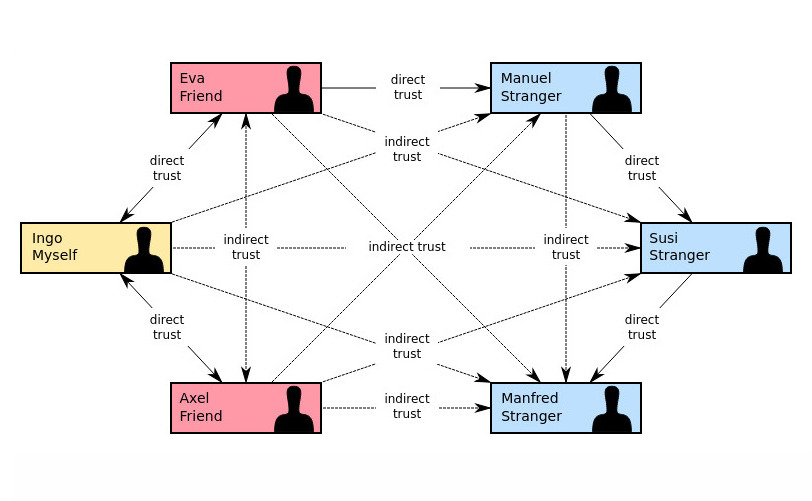
\includegraphics[width=0.45\textwidth]{i/weboftrust.jpg}
  \caption{Web of Trust, Source: Wikipedia}
\end{figure}


%% \subsection*{Philosophy of Key Management}
\subsection*{Web of Trust}

While the private key is kept secret,
the public key is shared with family and friends and acquaintances, and
is used by them to encrypt inbound messages by the user.
The core idea and the philosophy of the GPG key management lies in what is know as
the \textbf{\textit{Web of Trust}}\cite{weboftrust}.
Instead of relying on a central authority, like a Public Key Infrastructure (PKI),
the Web of Trust depends on individuals couching for each other's identities. 
The user essentially trusts the public key of the people they know,
and those friends that trust the user can extend their trust to those keys as well.
In other words, indirect trust will complement direct trust.


\begin{figure}
\centering
  
\includegraphics[width=0.45\textwidth]{i/GNU.jpg}
  \caption{GPG: copyleft under GNU GPL (GNU General Public License) 
  }
\end{figure}


\subsection*{Key Signing}
What does the process of Alice publicly acknowledging that \textit{``Alice trusts Bob''} involve?
By publicly signing Bob's public key,
Alice confirms that she believes that the public key authentically belongs to Bob.
Now Zoe trusts Alice and signs Alice's public key, and the same time
she gains some confidence in the authenticity of Bob's public key.
With time, the more Zoe's friends and others sign Bob's public key,
the greater will be the public's trust in the authenticity of Bob's key.
In this fashion,
continued key-signings progressively creates a web of interconnected trust
relationships.\cite{weboftrust}

\subsection*{Key Exchange}
Trust does not have to be exclusively over friends.
In fact, many users meet in-person and then exchange public keys and digitally sign each other's public keys.
There are at times social gatherings and parties with the main theme of
acquiring new friends and exchanging public keys with them.
The structure of such a Web of Trust is therefore decentralized and
community-driven.\cite{keysigningparty}

%% \begin{figure}
%% \centering
%%   
\includegraphics[width=0.45\textwidth]{i/GnuPG.jpg}
%%   \caption{GNU Privacy Guard}
%% \end{figure}


\begin{figure}
\centering
  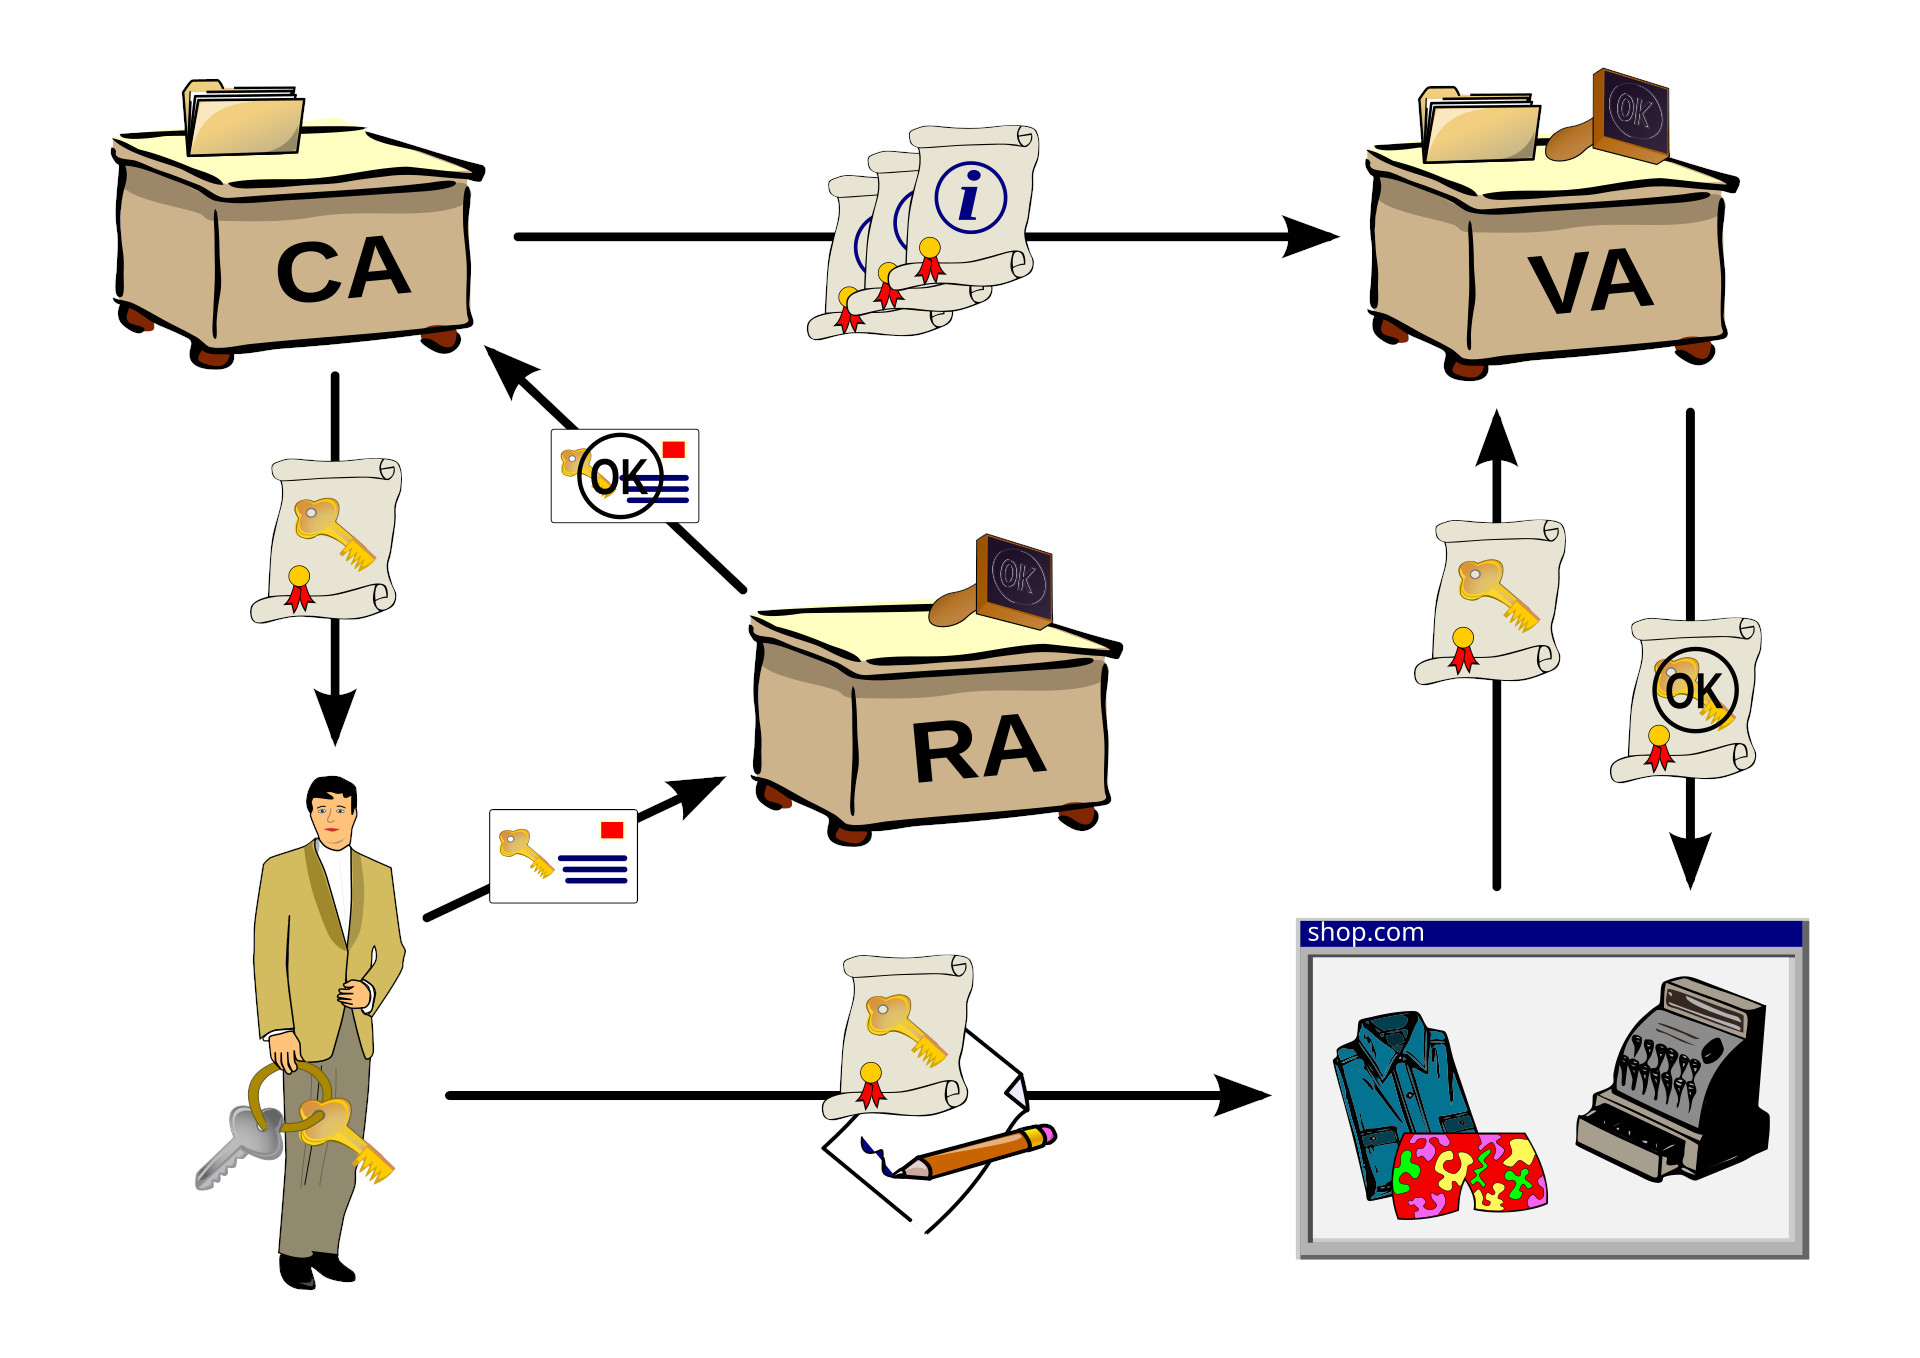
\includegraphics[width=0.45\textwidth]{i/PKIwikipedia.jpg}
  \caption{Public Key Infrastructure: Wikipedia}
\end{figure}


\section*{Public Key Infrastructure}
The public key infrastructure wholly relies on
Certificate Authorities (CAs).
CAs are ``trusted'' entities that issue and manage digital certificates, and
verify the identity of certificate applicants.\cite{whatareCA}
Although many intermediate CAs exist, they all rely on the
\textit{root certificates}
issued by 
\textit{root certificate authorities,}
in other words the top-level CAs,
which are supposed to be the foundation of trust in the PKI hierarchy.
This system at its core relies on
\textit{chain of trust}
and
\textit{delegation of authority.}

Although the exact numbers fluctuate,
there are only a little over a dozen main commercial certificate authorities, including:
DigiCert,
Sctigo,
GoDaddy,
GlobalSign, etc;
but numerous governmental certificate authorities, including:
U.S. Treasury Root Certification Authority (TRCA),
U.S. Treasury Operational Certification Authority (TOCA),
NASA Operational Certification Authority (NOCA),
Social Security Administration Certification of Authority (SSACA),
Department of Homeland Security Certification Authority (DHSCA), etc.\cite{CA}





\section*{Trusting Central Authority}
It all boils down to trust.
And trust can only be based on history and track record.
In this paper, we will include historical cases in and outside the US.
This history intricately elucidates the practical, legal, and ethical issues
surrounding reliance on a few ``trusted'' root authorities.
We will begin with evaluating 
the track record of commercial certificate authorities
and after that the track record of governmental certificates of authority.
Here are a few examples of the failure of the centralized trust systems involving commercial entities:\cite{CAfailure}

\subsection*{DigiNotar 2011}
This Dutch CA was compromised and fake certificates were issued and used for ``man-in-the-middle'' attack against Iranian Gmail users.
The result was DigiNotar's bankruptcy and a significant loss of trust in this centralized system of certification.\cite{diginotar}

\subsection*{Symantec 2015, 2015, 2017}
Symantec gained notoriety for not once but even while on probation issued over 100 bogus certificates, leading to 
Symantec ultimately being distrusted by all major platforms due to malfeasance. 
Symantec sold its business and was re-branded as DigiCert,
which is still one of the main issuers of certificates.\cite{digicert}

\begin{figure}
\centering
  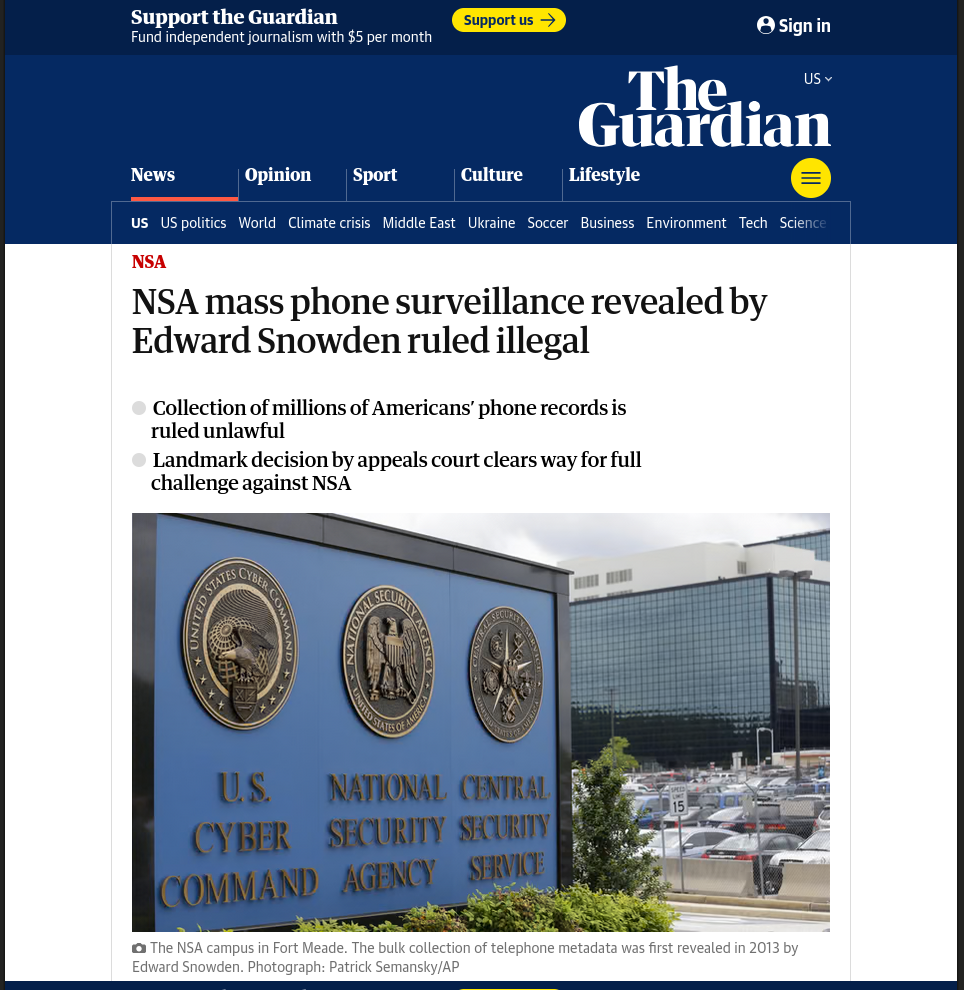
\includegraphics[width=0.45\textwidth]{i/illegal.png}
  \caption{NSA mass surveillance ruled illegal: Guardian 2015
  }
\end{figure}



\subsection*{WoSign 2015, 2016, 2017}
WoSign and its subsidiary were caught backdating certificates and engaging in other improper practices.\cite{CAfailure}


The list of the ways and incidents, where commercial entities have historically failed and betrayed the public trust is long \cite{CAfailure} \cite{CAfailure2}.
On the other hand, outside the realm of commercial entities,
incidents and scandals involving US government agencies and abuse of power in connection to their claimed
authority to issue certificates is also eye-opening.
Such incidents involving the misuse of their certification authority includes the following:


\subsection*{NSA 2013}
Widespread illegal surveillance of not only foreign nationals but US citizen by the NSA, that was brought to light by Snowden documents in 2013,
including man-in-the-middle attacks,
fake websites,
that received traffic re-directed from NY ATT-server closets,
interception of protected information,
and injection of poisoned data.
The Snowden documents also revealed NSA's ability to decrypt current \textit{commonplace}
encryption protocols, that they had previously falsely claimed to be secure.\cite{snowden}

\subsection*{Crypto AG, Operation Rubicon}
For decades the CIA and the German BND secretly owned and controlled the Swiss Company Crypto AG and distributed devices rigged with backdoors for the purpose of
eavesdropping worldwide\cite{rubicon}.

\begin{figure}
\centering
  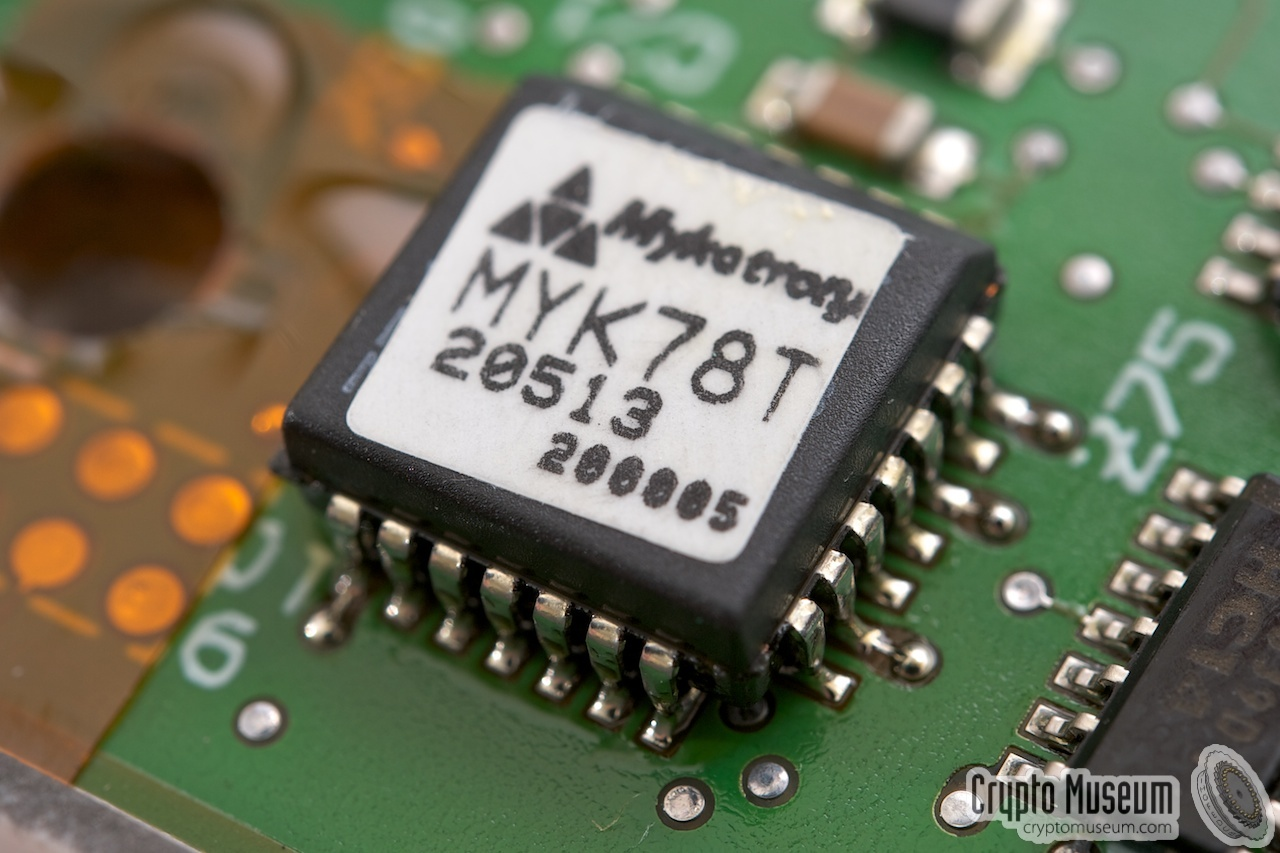
\includegraphics[width=0.45\textwidth]{i/clipper.jpg}
  \caption{Clipper Chip: Crypto Museum \cite{clipper}}
\end{figure}



\subsection*{Clipper Chip 1990}
The NSA developed a backdoored \textit{Clipper Chip}
with a compromised escrow key, that would allow illegal surveillance by the government\cite{clipper}.

\subsection*{Dual Elliptic Curve Deterministic Random Bit}
This was a backdoored cryptographically insecure random number generator promoted by the NSA, and
this illegal activity only came to light with Edward Snowden's 2013 revelations\cite{dual}.


\section*{Legal and Ethical Perspectives}
The main philosophical, socio-political, legal, and ethical questions arising from these 
complex, multilayered context are as follows:

Does this illegal surveillance constitute beneficence or malfeasance.
What cross-relationships exist among these various issues?
Should a US citizen be happy, if a powerful government, a metaphorical all-knowing parent, uses its might and all its tools,
including legal and illegal devices and strategies, to stay in power, to protect the status quo and the current state of
an uneven distribution wealth among US citizens,
and makes decisions for its naive children,
and continues to pursue
\textit{full spectrum dominance}
and to further the flourishing of 
\textit{American Exceptionalism}?
Should a US citizen be happy, if
a real-life Jack Nickelson poignantly and loudly exclaims
``You want The Truth? You can't handle The Truth!''
OR, should a US citizen demand
real participation in the decision-making process,
so that she or he can represent and protect their specific interests;
as opposed to the make-belief of soft-money-accepting elected officials voting against the interests of the average citizen and in favor of the billionaires at every turn?
Should a US citizen demand transparency and accountability?
Should a US citizen insist on the \textit{division of powers}
and be mortified to see all three branches rolled into one and in the clutches of a small, powerful, mostly unelected elite.
Should a US citizen worry about the un-free future awaiting his or her children in this neo-feudalistic social system?


\section*{Multilayered Ethical Concepts and Perspectives}

After applying these contrasting ethical and legal concepts one can finally recognize the nuanced
cross-relations among these diametrically opposed view-points and philosophies,
each one having very different implications which we must consider.

It is only after gaining a more comprehensive world-view, that a US citizen would truly be able to give an informed answer to the question:
Is it okay, if Big Brother\cite{1984} reads my emails, listens to my phone calls, collects every bit of information available about
my profile, either directly or through Palantir in a round-about fashion to circumvent existing laws that protect civil liberties?
Should I or my children, one day develop the courage to become politically active and participate in some pro-peace movement, would
Big Brother descend upon my life (or their lives) and destroy it all in a flash?

It is my position, being fully aware of all objections on the other side, that freedom trumps servitude, and I am confident, that I can reasonably defent
my position against all those who woould objection, specifically those who dishonestly use the cudgel  ``but what about national security.''
It is partly in this context,
and while considering various aspects of this complex issue, 
that the questions regarding cryptography, secure communications,
Web of Trust versus centralized certificate authorities should be pondered upon.
But first let us look at the concept of ``the government.''

What are the constituent \textit{parts} of the government?
If we dissect this entity, we will recognize, that it consists of
\textit{individual human beings},
the atomic units of its composition.
The government constitutes a complex system and, like all complex systems exhibits, \textit{emergent behavior}.
This emergent behavior is however a direct function of the mode of operation of its atomic subunits, namely the individuals.
So first, we have to understand how the subunits of this bureaucracy function.
I believe, that Hannah Arendt's insight can greatly assist us in exploring the
psyche of each one of these atomic subunits,
the modus operandi of each bureaucrat.
Only then can we shed light on the multi-layered relationship of this super-organism.
But, who was Hannah Arendt?


\begin{figure}
\centering
  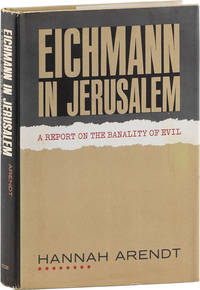
\includegraphics[width=0.30\textwidth]{i/banality.jpg}
  \caption{Hannah Arendt: The Banality of Evil}
\end{figure}


\section*{Hannah Arendt}
Hannah Arendt was a political theorist,
who in 1961 covered the trial of Adolf Eichman, a key Nazi SS officer organizing
the mass murder of communists and socialists and Jews.
In her book, The Banality of Evil,
she describes, that she expected to see a monstrous, hate-filled figure.
Instead what she found, was a pedantic bureaucrat, who was not driven by ideological fever or sociopathic malice,
but by the desire to fit in, obey orders, and be efficient.
She saw a cog in the machine that was incapable of independent judgment and
lacked the capacity to see the long-term consequences of his actions.
In other words, although his actions were heinous, his motivations were petty and ordinary.
Eichman's story showcased how ordinary people can commit extraordinary atrocities.
The 2023 movie \textit{The Zone of Interest} also
builds on the main theme of The Banality Evil.

So how can the ordinary man not become a cog in a machinery
that aims to destroy freedoms, including the freedom of speech, and
violate the civil rights of ordinary citizens just like this very ordinary man,
who only to aims to fit in, to obey, to be a team-player, and to be an obedient citizen?

\section*{The Courage to Think and to Speak}
The answer to the above question is this:
He must think. He must think freely. He has the moral duty to free his thought.
He has the ethical duty to read and to educate himself.
Towards his own progeny, he has the ethical duty to be brave. Brave to read, brave to learn, and brave to think.
A good citizen is morally obligated to grow.
The next question is what environment is particularly conducive to growth,
and what role does open and free social discourse play in this process of maturation?
What forces oppose free social discourse?


\section*{Opposing Free Social Discourse}
What is the historical precedence, when it comes to suppression of free speech? Are there any examples?

\begin{figure}
\centering
  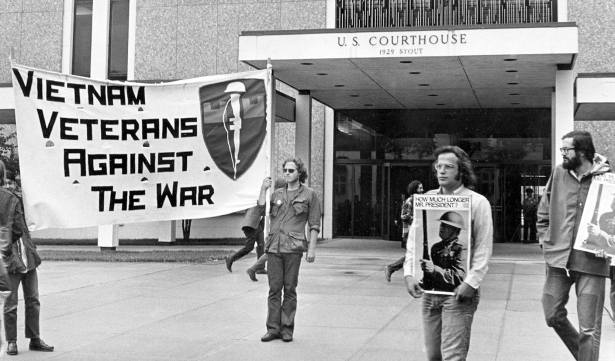
\includegraphics[width=0.45\textwidth]{i/vwv.jpg}
  \caption{Vietnam War Veterans, ``Peace is Dignity'' 1966
  }
\end{figure}


\subsection*{Vietnam War Era}
During the Vietnam War the government engaged in extensive surveillance
of anti-war activists and civil rights leaders.
The FBI routinely disrupted and attempted to discredit dissent group using legal and illegal means (COINTELPRO)\cite{cointelpro}.
These activities included wiretapping, infiltration, and spread of disinformation.
These attacks on free speech had a very significant chilling effect and successfully suppressed US citizens' constitutional rights,
including freedom of speech and freedom of assembly\cite{cointelpro}.


\begin{figure}
\centering
  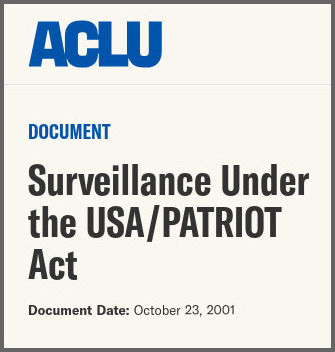
\includegraphics[width=0.45\textwidth]{i/pa.jpg}
  \caption{ACLU Document: 2001\cite{ACLU}
  }
\end{figure}


\subsection*{Patriot Act}
The Patriot Act has undoubtedly been the single most intrusive action ever undertaken
by the US government against US citizens.
Its chilling effect on free speech does not need to be belabored.
National Security Letters are used to subpoena records without any judicial oversight and the accompanying
gag order prevents the recipients from notifying the citizens, peace activists and the like, that they have been targeted.
The intrusion and pace of violation of constitutional rights of the citizens has significantly be increased by the introduction of \textit{fusion centers}\cite{fusion},
where agencies share data.
No meaningul protection for citizens' right to privacy exists.
The chilling effects of such pervasive and invasive surveillance is undeniable\cite{ACLU}.

\vspace{-6mm}

\section*{Conclusion: GPG Facilitates Social Discourse}
So how can GNU Privacy Guard technology facilitate freedom of speech and encourage social discourse?
Just as invasive and pervasive surveillance has a chilling effect on communication among friends and family,
protection against such unconstitutional intrusion would encourage friends and people who think alike to express themselves more freely
and exchange ideas, without the fear of suddenly being targeted, and seeing their life and livelihood evaporate in a flash in front of their eyes.
Typically, however, citizens only engage in deep philosophical and political discourse with their close family members and friends and not necessary
when exchanging business email or assisting their accountant to complete tax forms.
Hence GPG only needs to be used for a limited number of communications between close friends;
communication that would otherwise not blossom and wither, when exposed to the destructive effect of surveillance.
In this digital age, widespread surveillance has created a modern-day panopticon.
People internalize the feeling of being watched. This leads to self-censorship and a reluctance to engage in dissenting or unconventional thought.
However, once citizens truly believe that they have exited the panopticon,
many will likely feel motivated to discuss social and budgetary matters;
issues that deeply affect their everyday lives.
Open debate on these matters is vital for democratic societies.
Informed citizens who freely express their opinions are better equipped to advocate for change and social progress\cite{yale}.


\section*{The Future: The Hybrid Method}
In the future likely hybrid methods will floursih.
Since the number of GPG keys that need to be exchanged and stored
grows with $O(n^2)$, realistically GPG and
the decentralized method of Web of Trust
should be the primary method of encrypting communication among friends and family members,
the inner circle,
since that conversation would likely include political discourse.
The fall-back method would still remain the centralized Root Certificate Authority validation of the identity of individuals and entities.
It is my now my position, that in this fashion an adequate breathing space can be created for US citizens,
who could then start engaging in free social and political discourse,
without fearing Big Brother's\cite{1984} devastating retaliation\cite{1984b}.


\textit{
\enquote{
Posterity will be the beneficiary. -- me}} 
\hfill
$\square$


%% \ensuremath{\square}
%% \unicode{x25A1}



















%% \begin{figure}[h!]
%% \centering
%%   
\includegraphics[width=0.40\textwidth]{i/iccsu.jpg}
%% %%   \caption{Web of Trust, Source: Wikipedia}
%% \end{figure}












\begin{figure}[h!]
\centering
  
\includegraphics[width=0.40\textwidth]{i/iccsu.jpg}
%%   \caption{Web of Trust, Source: Wikipedia}
\end{figure}


\vspace{-10mm}

\section*{Acknowledgments}
My heartfelt thanks go to Dr. Joseph Paige,
Ombudsperson at Central Connecticut State University,
for his warm encouragement and insightful advice,
which have been a great comfort and assistance during my final semester.
I would also like to thank Professor Chad Williams for his
invaluable support and guidance throughout my graduate studies.


%----------------------------------------------------------------------------------------
%	REFERENCE LIST
%----------------------------------------------------------------------------------------

%%%% this command added later %%%
%\onecolumn


\fontsize{8}{8}\selectfont
\fontsize{7}{7}\selectfont


\begin{thebibliography}{99} % Bibliography - this is intentionally simple in this template

  
%% \bibitem[Figueredo and Wolf, 2009]{Figueredo:2009dg}
%%   Figueredo, A.~J. and Wolf, P. S.~A. (2009).
%%   \newblock Assortative pairing and life history strategy - a cross-cultural study.
%%   \newblock {\em Human Nature}, 20:317--330.

\bibitem{wikiGPG}
  ``GNU Privacy Guard.'' Wikipedia, Wikimedia Foundation, As of 21 March 2025, https://en.wikipedia.org/wiki/GNU\_Privacy\_Guard

\bibitem{firstamendment}
  U.S. Constitution - First Amendment | Resources | Constitution Annotated | Congress.Gov | Library of Congress, constitution.congress.gov/constitution/amendment-1/. Accessed 21 Mar. 2025. 

\bibitem{humanrights}
  “United Nations Human Rights System - Global Freedom of Expression.” Global Freedom of Expression, 2019, globalfreedomofexpression.columbia.edu/law-standards/united-nations-human-rights-system/.

\bibitem{whitney}
  “Whitney v. California | the National Constitution Center.” National Constitution Center – Constitutioncenter.org, 2022, constitutioncenter.org/the-constitution/supreme-court-case-library/whitney-v-california.

\bibitem{goering}
  DWOOD. “Intellectual Freedom Quotes.” About ALA, 1 Aug. 2017, www.ala.org/aboutala/intellectual-freedom-quotes.

\bibitem{wernerkoch}
  Wikipedia Contributors. “Werner Koch.” Wikipedia, Wikimedia Foundation, 5 Jan. 2025.


\bibitem{openpgp}
  “Pretty Good Privacy.” Wikipedia, 5 Oct. 2022, en.wikipedia.org/wiki/Pretty\_Good\_Privacy\#OpenPGP.

\bibitem{rfc4880}
  Callas, J., et al. “OpenPGP Message Format.” Www.rfc-Editor.org, 1 Nov. 2007, www.rfc-editor.org/rfc/rfc4880, https://doi.org/10.17487/RFC4880.


\bibitem{weboftrust}
  Wikipedia Contributors. “Web of Trust.” Wikipedia, Wikimedia Foundation, 4 June 2019, en.wikipedia.org/wiki/Web\_of\_trust.

\bibitem{keysigningparty}
  Wikipedia Contributors. “Key Signing Party.” Wikipedia, Wikimedia Foundation, 20 July 2024.

\bibitem{whatareCA}
  Archiveddocs. “What Are ca Certificates?: Public Key; Security Services.” Learn.microsoft.com, 9 Aug. 2010, learn.microsoft.com/en-us/previous-versions/windows/it-pro/windows-server-2003/cc778623(v=ws.10)?redirectedfrom=MSDN.

  
\bibitem{CA}
  Wikipedia Contributors. “Certificate Authority.” Wikipedia, Wikimedia Foundation, 9 Jan. 2020, en.wikipedia.org/wiki/Certificate\_authority.


\bibitem{CAfailure}
“Timeline of Certificate Authority Failures - SSLMate.” Sslmate.com, sslmate.com/resources/certificate\_authority\_failures.

\bibitem{CAfailure2}
  Hadan, Hilda, et al. “A Holistic Analysis of Web-Based Public Key Infrastructure Failures: Comparing Experts’ Perceptions and Real-World Incidents.” Journal of Cybersecurity, vol. 7, no. 1, 1 Jan. 2021, https://doi.org/10.1093/cybsec/tyab025.
  
\bibitem{snowden}
  Wikipedia Contributors. “Edward Snowden.” Wikipedia, Wikimedia Foundation, 16 Mar. 2019, en.wikipedia.org/wiki/Edward\_Snowden.

\bibitem{rubicon}
  “Rubicon.” Www.cryptomuseum.com, www.cryptomuseum.com/intel/cia/rubicon.htm.

\bibitem{clipper}
  “Clipper Chip.” Www.cryptomuseum.com, www.cryptomuseum.com/crypto/usa/clipper.htm.


\bibitem{dual}  
  “Dual\_EC\_DRBG.” Wikipedia, 13 Mar. 2022, en.wikipedia.org/wiki/Dual\_EC\_DRBG.

\bibitem{diginotar}
  Wolff, Josephine. “How a 2011 Hack You’ve Never Heard of Changed the Internet’s Infrastructure.” Slate Magazine, 21 Dec. 2016, slate.com/technology/2016/12/how-the-2011-hack-of-diginotar-changed-the-internets-infrastructure.html.


\bibitem{digicert}
  “DigiCert to Acquire Symantec’s Website Security Business.” Digicert.com, 6 Mar. 2024, www.digicert.com/blog/digicert-to-acquire-symantec-website-security-business. Accessed 22 Mar. 2025.



\bibitem{cointelpro}
  FBI. “COINTELPRO.” FBI, 2020, vault.fbi.gov/cointel-pro.



\bibitem{ACLU}  
  “PATRIOT Act Fears Are Stifling Free Speech, ACLU Says in Challenge to Law | American Civil Liberties Union.” American Civil Liberties Union, 20 Sept. 2005, www.aclu.org/press-releases/patriot-act-fears-are-stifling-free-speech-aclu-says-challenge-law.

\bibitem{fusion}
  https://www.aclu.org/news/national-security/secret-domestic-surveillance-program-about-get-pulled-out-shadows
  
\bibitem{yale}
  https://politicalscience.yale.edu/publications/open-democracy-reinventing-popular-rule-twenty-first-century


\bibitem{1984}
  Wikipedia Contributors. “Nineteen Eighty-Four.” Wikipedia, Wikimedia Foundation, 16 Feb. 2019, en.wikipedia.org/wiki/Nineteen\_Eighty-Four.

\bibitem{1984b}
  George Orwell. George Orwell’s 1984. Internet Archive, archive.org/details/GeorgeOrwells1984.

  
\end{thebibliography}

%----------------------------------------------------------------------------------------



\end{document}


